%!TEX root = ../main.tex

\chapter{Multirobot search strategy\label{chap:methods_robotics}}
This chapter presents a multirobot search strategy for a group of \ac{UAV}s equipped with the Compton camera for online estimation of sources of ionizing radiation, 
which is based on the \ac{MLEM} method described in the previous chapter.
The search method takes a) the current \ac{MLEM} estimate of radiation intensity and b) the sensitivity of detection of the whole multi-robot system and compute future actions of the \ac{UAV}s.
We assume that the search mission is performed in open area without obstacles.
Objectives and requirements for the proposed search method and as well as its individual parts are presented in this chapter.
%Section \ref{sec:obj} describes the objectives and requirements for such method.
%The whole system is described in the next section, as well as individual components of the system.
\section{Objectives\label{sec:obj}}
%The \ac{MLEM} method proposed in the previous chapter provides the maximum likelihood estimate of the measured data.
%When the number of detected Compton events is low, the maximum likelihood estimation method might suffer of inaccurate 

\subsection{Measure as much data as possible}
As stated before, the emission of $\gamma$ particles as well as the detection of Compton events are stochastic processes.
The intensity of radioactive emission follows the inverse square law, which means that it decreases as the distance from the source increases.
Due to the small size of the detector, large distances between \ac{UAV}s and sources of ionizing radiation, and the fact that only $\approx 2\%$ of $\gamma$ particles reaching the detector are detected by the Compton camera (on average), the number of detected events is limited.
The accuracy of the \ac{MLE} method depends on the number of detected Compton events.
If the number of detected cones is low, the \ac{MLE} method might converge to false detections since the particle could originate from any position on the surface of the Compton cone.
To accurately localize the sources of ionizing radiation, the \ac{UAV}s should collect as many measurements as possible.
This requires the \ac{UAV}s to fly as close as possible to the currently most likely source estimates to either confirm or disprove the presence of the radioactive source at the given position.
It is also desired that the drones stay in motion (instead of hovering above the points of interest), since measurements from different angles are beneficial for sources localization.

\mycomment{% %%{
  As stated before, the emission as well as the detection of Compton events are stochastic processes.
  The intensity of radioactive emission decreases with inverse square law as the distance from source grows.
  Because of the small size of the detector, large distances between \ac{UAV}s and sources oinizing radiation and the fact that only $2 \%$ of $\gamma$ particles that reach the detector are detected by the Compton camera, the number of detected events is limited.
  The accuracy of \ac{MLE} method from definition depends on the number of detected Compton events.
  When the number of detected cones is low, the \ac{MLE} method might converge to false detections (since the particle could originated from any position on the surface of Comtpon cone).
  To measure more data, the \ac{UAV}s should collect as many measurements as possible.
  It requires the \ac{UAV}s to fly as close as possible to the currently most likely source estimates to either confirm or disprove the presence of the radioactive source at the given position.
}% %%}

\subsection{Search for unobserved sources of ionizing radiation}
The sensitivity vector $\mathbf{s}$ described in the previous chapter specifies the probability that a particle emitted at certain position is detected.
The sensitivity of detection can be therefore seen as
\begin{equation}
  s_{j} = P(\mathrm{detected\ by\ the\ UAV\ system} | \mathrm{emitted\ from} \ j),
\end{equation}
which can be interpreted as a coverage of the area of interest, specifying how much has been point $j$ explored.
The autonomous \ac{UAV}s should control their motion in the way that the whole area is covered.
In another words, the minimum value of sensitivity $\mathrm{min}(s_{j})$ among all positions in the search space should be as high as possible to increase the chance of observing sources that were not yet detected.

\subsection{Active search strategy}
Two general strategies for exploring an area of interest by a group of autonomous \ac{UAV}s and for measuring data and estimating sources of ionizing radiation are considered --- offline and online.
In offline search, the \ac{UAV}s typically follow predefined paths and collect measurements, that are processed all at once after the flight. 
In online search, the estimation process is performed online and the \ac{UAV}s may react accordingly to the current output of the radiation mapping method.
Incorporating the output of the mapping method into the feedback control loop 
might lead to better estimate (since more measurements might be acquired) and fasten the search time.
In general, an active search strategy allows the group of \ac{UAV}s to use its full potential, therefore it is desired for the given task.

\mycomment{% %%{
\subsection{Motivation for mlem}
Neco o tom yze i negativni mereni jsou dulezity
  The emission of $\gamma$ particles as well as the detection of Compton events are stochastic processes.
  Only a small fraction of emitted $\gamma$ particles are detected by the small \ac{pix} sensor located several meters from the radioactive source.
  Moreover, the intensity of radioactive emission decreases with the inverse square law as the distance from the source grows.
  Taking into account also ther properties of the ionizing radiation and the detection process, the acquired measurements are highly dependent on the trajectories of the \ac{UAV}s performing the search mission.
  The \ac{UAV}s might be controlled in two ways: they can either a) follow some trajectory that cover the whole area of interest uniformly or b) the trajectory of the \ac{UAV} is arbitrary and the coverage of the space is not uniform.
  However, it doesn't use the whole potential of small and agile \ac{UAV}s carrying the Compton camera.
  In b) approach, it is required 
}% %%}

\mycomment{% %%{
  \subsection{Centralized vs. decentralized}
  The multirobot systems can be classified into two groups: centralized and decentralized.
  In a centralized approach, a central control unit is responsible for coordinating the actions of all the robots in the network. 
  This centralized system can provide global information to each robot, enabling them to make more informed decisions based on the overall state of the system.
  On the other hand, it is vulnerable to single points of failure and it requires reliable communication between each agent and the central unit.
  In decentralized system, each robot operates independently, making decisions based on local information and communication with other robots in the network. 
  This approach can provide increased fault tolerance and can be more adaptable to changing conditions. 
  However, the lack of a central control unit can make it challenging to ensure that all robots are efficiently working towards a common goal.
}% %%}

\section{System design description}
\subsection{Task specification}
The proposed search strategy is based on the objectives described above --- the group of \ac{UAV}s should autonomously explore the area of interest with no previous knowledge about number, activity or position of sources of ionizing radiation and localize such sources as fast as possible.
The operation of the \ac{UAV}s is divided into two main tasks:
\begin{itemize}
  \item \textbf{exploration}: the drones should explore the area of interest and increase the chance that none of the sources of $\gamma$ particles would be unobserved,
  \item \textbf{exploitation}: the drones should exploit positions where \ac{MLEM} mapping method estimated some emission activity to either confirm the hypothesis and collect more measurements or disprove it (in general, increase accuracy of the estimation).
\end{itemize}
The exploration-exploitation dilemma is solved by dedicating each \ac{UAV} to either exploration of exploitation task.
%\subsection{Assumptions}
%It is assumed that 
%a) a communication via wireless network is provided, 
%b) the mission is performed in outdoor environment with no obstacles, 
%c) the sources of ionizing radiation are located somewhere on the ground, that is for simplicity assumed to be a flat plane.

\subsection{Multirobot architecture}
The multirobot systems can be classified into two groups: centralized and decentralized.
In a centralized approach, a central control unit is responsible for coordinating the actions of all the robots in the network. 
This centralized system can provide global information to each robot, enabling them to make more informed decisions based on the overall state of the system.
%On the other hand, it is vulnerable to single points of failure and it requires reliable communication between each agent and the central unit.
In decentralized system, each robot operates independently, making decisions based on local information and communication with other robots in the network. 


The centralized multirobot architecture is used in this project.
The visualization of the system architecture is presented in \autoref{fig:sysarch}.
The \ac{UAV}s are communicating via wireless \textbf{Wifi} network.
The amount of information shareable via such network is limited.
Therefore all the \ac{MLEM} computations and running on a ground station and the \ac{UAV}s and ground station share the minimal amount of information possible.
All the \ac{UAV}s send its current position and future position as a custom \ac{ROS} message (with frequency $\SI{5}\hertz$) and newly detected Compton cones.
The ground station processes the measurements and command the \ac{UAV}s by sending non-colliding path for each of them via the wireless network.
The centralized approach have several advantages in this scenario:
the \ac{MLEM} estimate is computed at once, not requiring to share or merge the map with other \ac{UAV}s via the wireless network or run the estimation onboard each drone separately.
The centralized task allocation and path planning is much more straightforward compared to the decentralized approach, where the agents would need to negotiate between each other.
\begin{figure}[!htb]
    \centering
    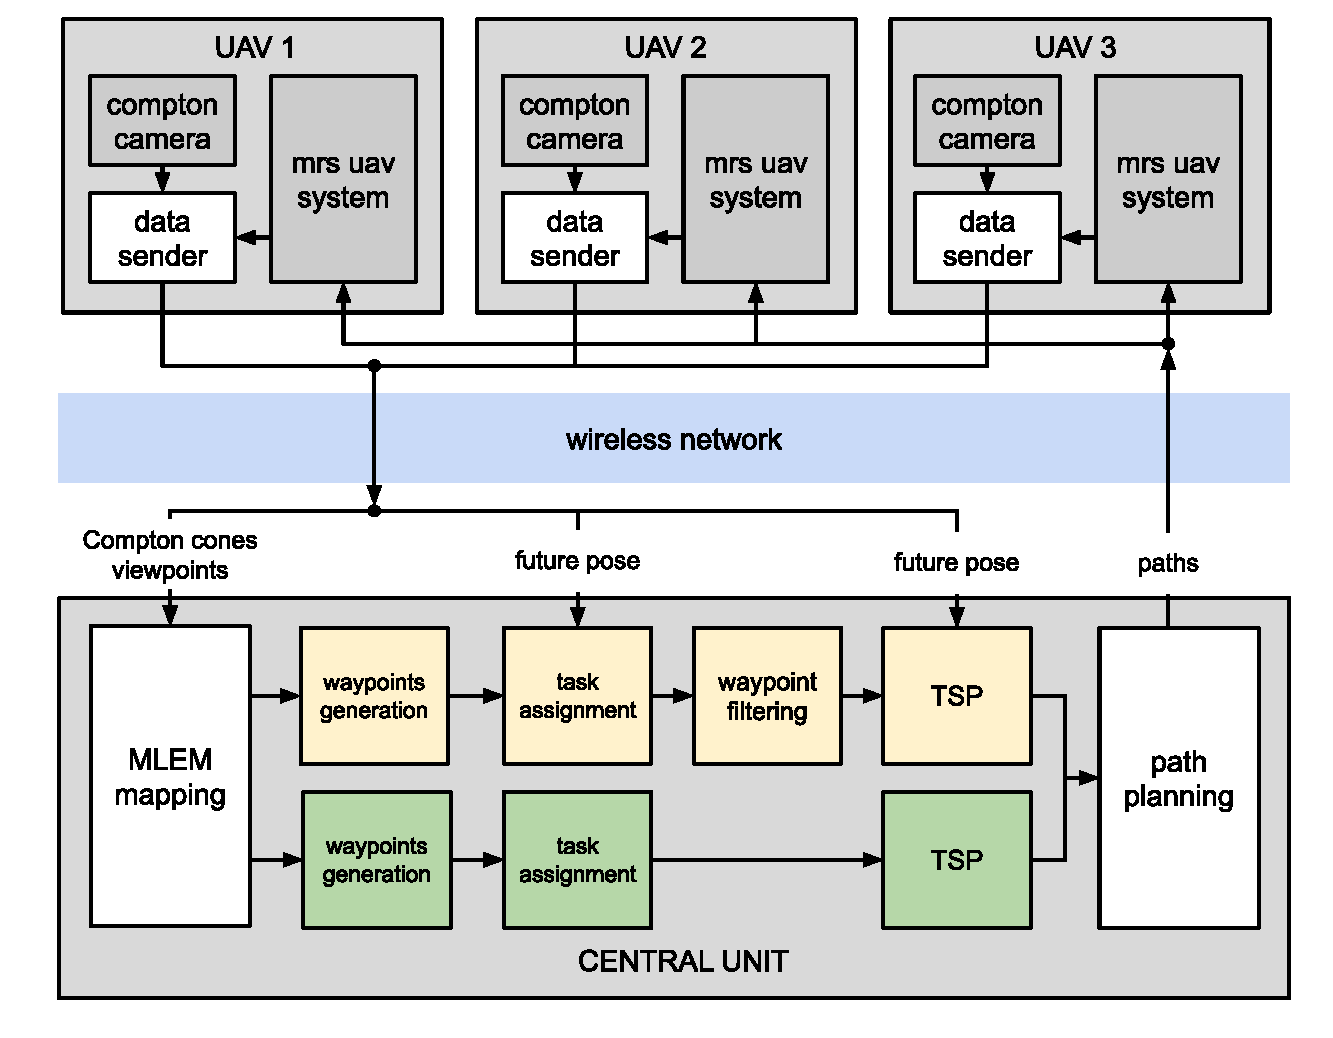
\includegraphics[width=0.99\textwidth]{./fig/photos/sysarch_new.eps}
    \caption{\centering The system architecture diagram. The search and planning method is composed of \ac{MLEM} radiation mapping node, waypoint generation, task assignment, waypoint filtering, optimal sequence deduction using \ac{TSP} and path planning. The exploration (green) and exploitation (yellow) waypoints are processed separately.}
    \label{fig:sysarch}
\end{figure}

\section{Search and planning strategy description}
%The system pipeline is composed of multiple components, as illustrated in \autoref{fig:sysarch}.
The central method responsible for search and planning strategy is composed of multiple components: 
\textbf{MLEM mapping}, \textbf{waypoints generation}, \textbf{task assignment}, \textbf{waypoint filtering}, optimal sequence of waypoints deduction using \textbf{\acf{TSP}} and \textbf{path planning}.
Each step of the system design is visualized in \autoref{fig:pipeline}.

The MLEM mapping node produces the current estimate of source intensities $\bm{\lambda}$ and current estimate of sensitivity $\mathbf{s}$, 
which are taken as input of the waypoint generation node (\ref{fig:pip1}).
The waypoint generation node assigns weights to the waypoints (\ref{fig:pip2}).
The filtered waypoints are then assigned to individual \ac{UAV}s (\ref{fig:pip3}).
To avoid revisiting the same point multiple times while ignoring others, the recently visited waypoints are filtered out in the next step (\ref{fig:pip4}).
All points assigned to one \ac{UAV} are connected into an optimal sequence (starting at the future position of the drone) using \ac{TSP} (\ref{fig:pip5}).
Finally, non-colliding paths are planned for all \ac{UAV}s (\ref{fig:pip6}).
The more detailed description of each individual step follows in the next sections.
%This design choice of course have some disadvantages as well.
%The centralized system is vulnerable to single point of failure and the communication between the ground station and all \ac{UAV}s must provided. 







% FIGURES STEPS of PIPELINE
\begin{figure}[!htb]% %%{

  \subfloat[\centering \textbf{waypoint generation} - detected local maxima of \ac{MLEM} estimate] {
    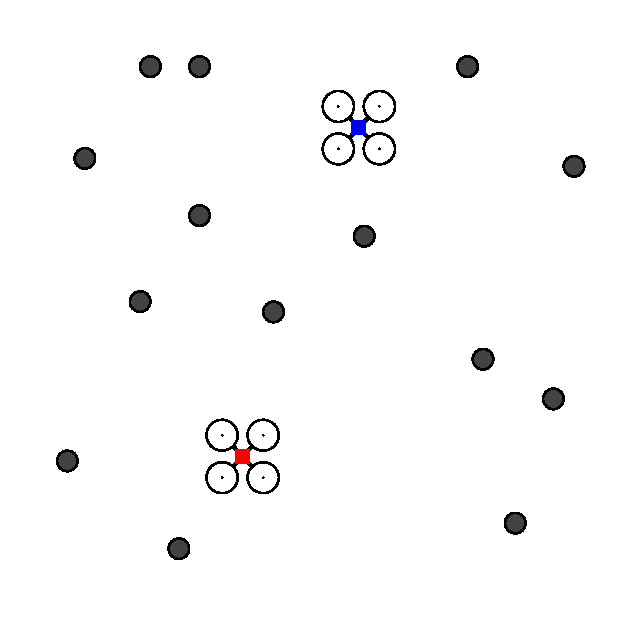
\includegraphics[width=0.3\textwidth]{./fig/photos/pip1.eps}

    \label{fig:pip1}
  }
  \subfloat[\centering \textbf{waypoint generation} - weighing and filtering] {
    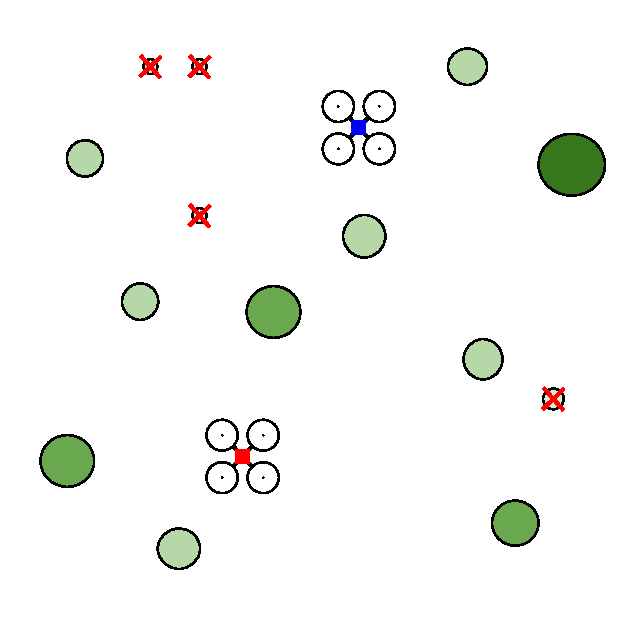
\includegraphics[width=0.3\textwidth]{./fig/photos/pip2.eps}
    \label{fig:pip2}
  }
  \subfloat[\centering \textbf{task assignment} - assigning waypoints to \ac{UAV}s] {
    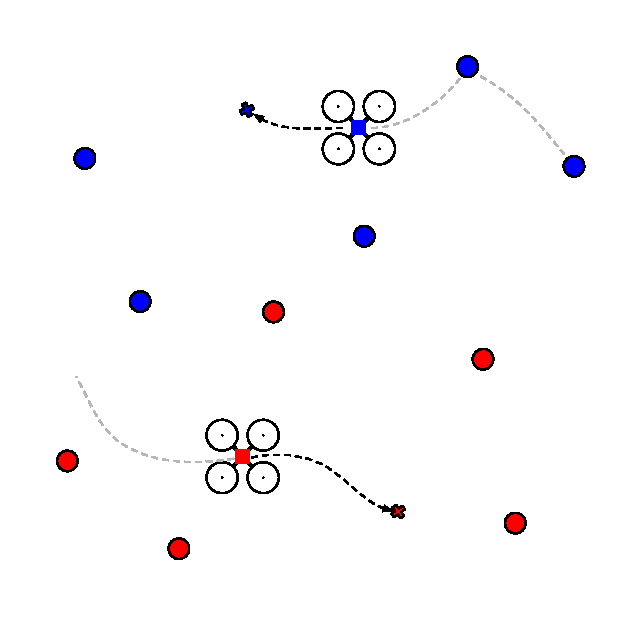
\includegraphics[width=0.3\textwidth]{./fig/photos/pip3.eps}
    \label{fig:pip3}
  }
  \newline
  \subfloat[\centering \textbf{waypoint filtering} - removal of recently visited waypoints based on short-term sensitivity] {
    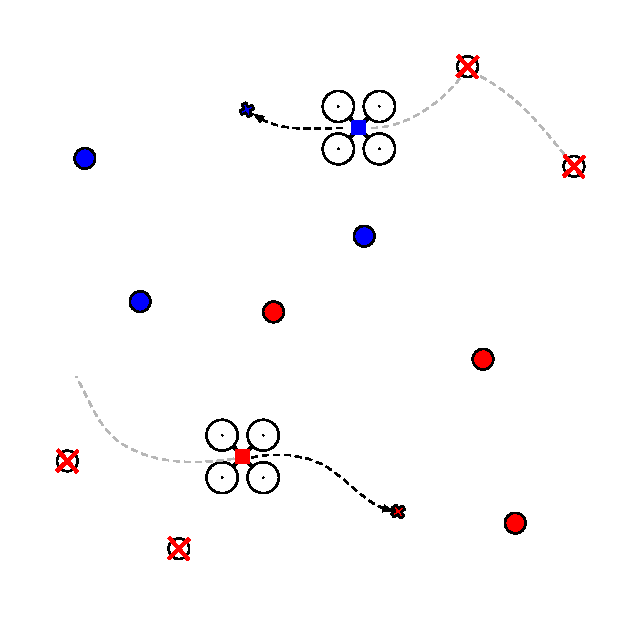
\includegraphics[width=0.3\textwidth]{./fig/photos/pip4.eps}
    \label{fig:pip4}
  }
  \subfloat[\centering \textbf{TSP} - optimal sequence determination] {
    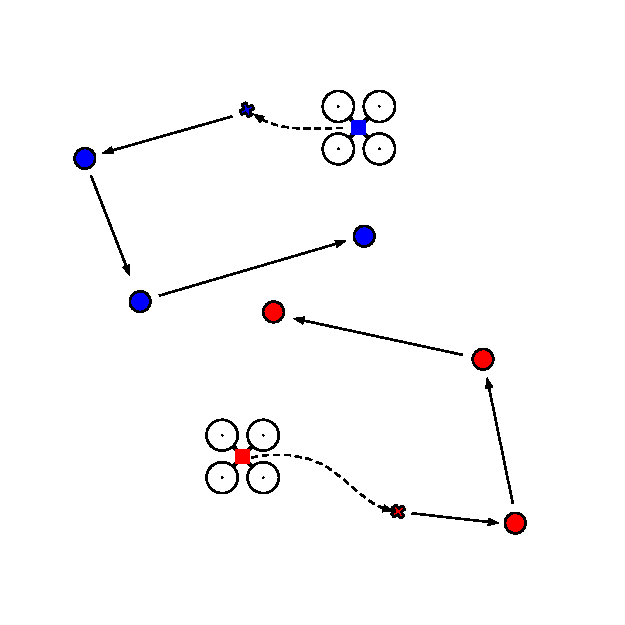
\includegraphics[width=0.3\textwidth]{./fig/photos/pip5.eps}
    \label{fig:pip5}
  }
  \subfloat[\centering \textbf{path planning} - find non-colliding paths connecting the waypoints] {
    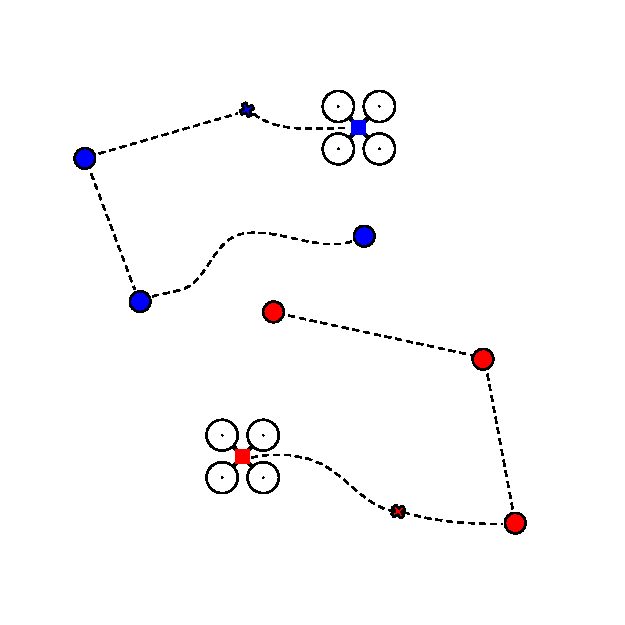
\includegraphics[width=0.3\textwidth]{./fig/photos/pip6.eps}
    \label{fig:pip6}
  }
  \caption{Individual steps of the system architecture. Waypoints are generated based on the current \ac{MLEM} estimate \protect\subref{fig:pip1}.
  The weighted and filtered waypoints \protect\subref{fig:pip2} are then assigned to individual \ac{UAV}s \protect\subref{fig:pip3}.
  The system prioritizes waypoints that were not recently visited \protect\subref{fig:pip4}.
  Finally, an optimal sequence of waypoints for each \ac{UAV} is determined using \ac{TSP} \protect\subref{fig:pip5} and the sequence of waypoints is passed to the planning node, that finds non-colliding paths for all \ac{UAV}s \protect\subref{fig:pip6}.}
  \label{fig:pipeline}
\end{figure}% %%}

%In the beginning, the exploitation waypoints are generated from the current \ac{MLEM} estimate ( \autoref{fig:pip1}).
%Each waypoint is assigned a weight and only subset of waypoints with highest weights are processed to the next step ( \autoref{fig:pip2}).
%The waypoints are assigned to the \ac{UAV}s using clustering method ( \autoref{fig:pip3}).
%The recently visited exploitation waypoints are removed in the next step ( \autoref{fig:pip4}).


\mycomment{% %%{
  \section{multirobot approach}
  The previous chapter presented the method for localizing sources of ionizing radiation.
  %Given the collected measurements, it can compute the maximum likelihood estimate of the sources locations.
  Moreover, the sensitivity computed in the \ac{MLEM} method provides information about how much has been the area explored by the compton cameras onboard the \ac{UAV}s.

  This motivates the search strategy described in this section:
  The movement of the \ac{UAV}s should be controlled in a way that they simultaneously perform the following tasks:
  \begin{itemize}
    \item \textbf{exploration} - explore the least explored maps in the area of interest and increase the chance that so far unobserved sources of radiation will be detected
    \item \textbf{exploitation} - fly where the radioactive sources are likely present (based on the current maximum likelihood estimate) to improve the accuracy of the estimate. 
  \end{itemize}

%The maximum likelihood approach requires collecting as many measurements as possible to make the estimate more accurate.
%At the same time, the drones should explore the unexplored area to increase chance that the estimation method won't miss any source of ionizing radiation.
%The task for the mutirobotic system can be summarized as follows:
%\begin{itemize}
%  \item \textbf{exploration} - explore the least explored maps in the area of interest
%  \item \textbf{exploitation} - acquire more measurements from areas, where the source of ionizing radiation is likely present
%\end{itemize}
}% %%}

\newpage



%%%%%%%%%%%%%%%%%%%%%%%%%%%%%%%%%
%%%%% WAYPOINTS GENERATION %%%%%%
%%%%%%%%%%%%%%%%%%%%%%%%%%%%%%%%%


\section{Waypoints generation}% %%{
\subsection{Exploitation}
\subsubsection{Local maxima filter}
The current estimate of ionizing radiation sources positions serves as an input for the waypoint generation method.
The map estimated by the \ac{MLEM} method is processed and local maxima of the map are detected.
Local maximum is a cell in the discretized map that has the highest value among all cells in its neighborhood. 
The size of the sliding window determining the neighborhood of each cell is a parameter that can be set.
The local maxima filter is illustrated in  \autoref{fig:filter}.

% filter%%{
\begin{figure}[!htb]
  \centering
  \subfloat[\centering input of the filter] {
    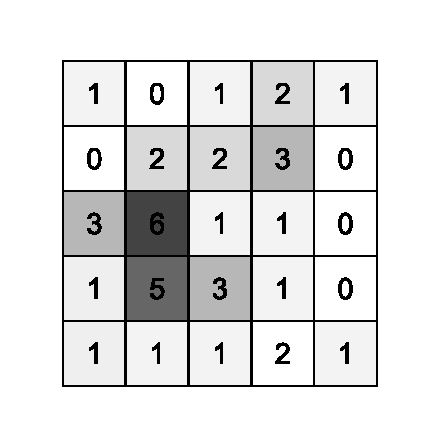
\includegraphics[width=0.2\textwidth]{./fig/photos/filter1.eps}

    \label{fig:fil1}
  }
  \subfloat[\centering filter window size 3] {
    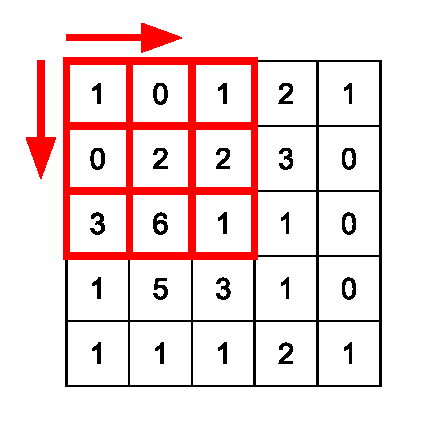
\includegraphics[width=0.2\textwidth]{./fig/photos/filter3.eps}
    \label{fig:fil2}
  }
  \subfloat[\centering detected local maxima] {
    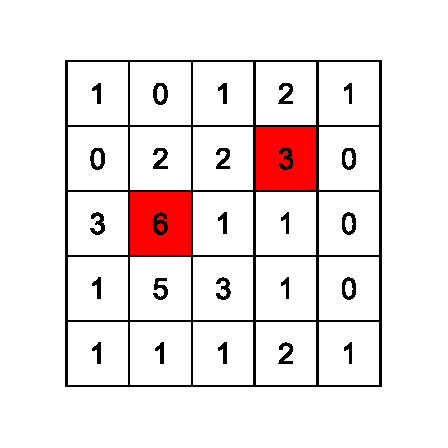
\includegraphics[width=0.2\textwidth]{./fig/photos/filter2.eps}
    \label{fig:fil3}
  }
  \caption{Local maxima filter demonstration}
  \label{fig:filter}
\end{figure}% %%}

\subsubsection{Waypoint weighting and filtration}
The waypoints associated with local maxima are weighted using following formula:
\begin{equation}
  w_{j_{weight}} = \frac{\lambda_{j}}{    s_{j_{normalized}} },
\end{equation}
where $s_{j_{normalized}} = \frac{ s_{j} }{ \underset{j}{\mathrm{max}}(s_{j})}$ is a sensitivity value normalized to range $[0, 1]$.
The purpose of the weighting step is following: it should prioritize the waypoints (local maxima) that are less explored (the sensitivity value is small compared to other waypoints).
The list of possible waypoints is then sorted from the highest $w_{j_{weight}}$ to the lowest.
Top $n$ waypoints based on the $w_{j_{weight}}$ are propagated further in the algorithm, the rest is ignored (parameter $n$ is set to $n = 10d$, where $d$ is number of drones used for exploitation).
The aim of filtering step is to remove the local maxima that were caused by noise in the \ac{MLEM} estimation.% %%}

\subsection{Exploration}
The task is to explore the map positions that have low sensitivity values (the probability that particle emitted from such position to be detected is low).
The process of generating waypoints for exploration is illustrated in  \autoref{fig:downsampling}.
The sensitivity vector $\mathbf{S}$ is downsampled by a mean filter with the stride equal to the filter window size.
The positions in the downsampled map are then sorted based on the mean sensitivity value.
Arbitrary percentage $p$ of the map poses with lowest sensitivity values is taken and exploration waypoints are generated in the centers of such downsampled map positions, as shown in  \autoref{fig:down3} for $p = 25\%$.

% downsampling%%{
\begin{figure}[!htb]
  \centering
  \subfloat[\centering input vector $\mathbf{S}$ in 2D] {
    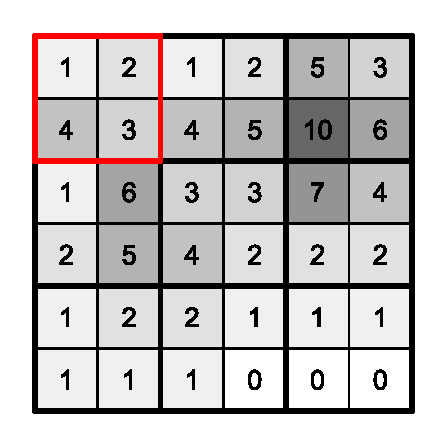
\includegraphics[width=0.25\textwidth]{./fig/photos/downsampling1.eps}

    \label{fig:down1}
  }
  \subfloat[\centering downsampled map (for window size and stride both equal 2)] {
    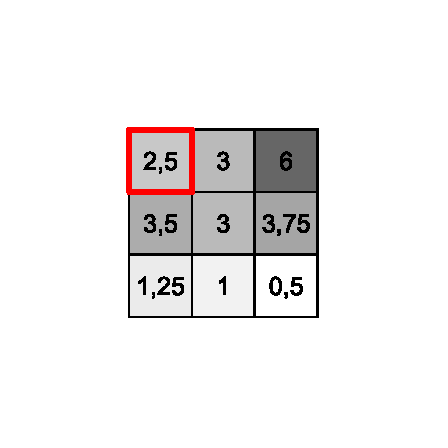
\includegraphics[width=0.25\textwidth]{./fig/photos/downsampling2.eps}
    \label{fig:down2}
  }
  \subfloat[\centering generated waypoints in the downsampled map for $p = 25\%$] {
    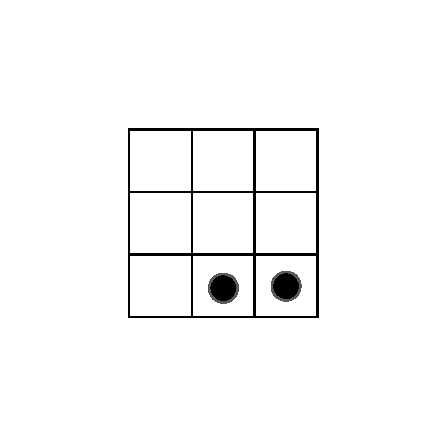
\includegraphics[width=0.25\textwidth]{./fig/photos/downsampling3.eps}
    \label{fig:down3}
  }
  \caption{Downsampling and waypoint generation process for exploration}
  \label{fig:downsampling}
\end{figure}% %%}


%%%%%%%%%%%%%%%%%%%%%%%
%%%%% CLUSTERING %%%%%%
%%%%%%%%%%%%%%%%%%%%%%%
\section{Clustering}% %%{
Clustering belongs to the group of unsupervised machine learning methods.
The goal of clustering is to partition the data into distinct groups (clusters), where data points within the same cluster are more similar to each other than to those in other clusters.
The euclidean distance is the measure of similarity used in this scenario.
The clustering algorithm of choice for the given task is \textbf{KMeans}, originally described in \cite{kmeans}.
The generated and filtered waypoints need to be assigned to the individual \ac{UAV}s. 
First step for that is clustering into groups, one group for each \ac{UAV} contributing to exploitation.

\subsection{KMeans algorithm}
The basic euclidean version of KMeans is defined as follows:
Let's denote data points to be clustered as $\{\mathbf{w}_{1}, \mathbf{w}_{2}, \dots , \mathbf{w}_{n}\}$.
The task is to assign each of the data points into one of the $k$ clusters, $\{C_{1}, C_{2}, \dots, C_{k}\}$.
Each cluster is represented by its centroid, $\mathbf{c}_{1}, \mathbf{c}_{2}, \dots, \mathbf{c}_{k}$.
The criterion function that should be minimized is then formulated as
\begin{equation}
  J = \sum_{i = 1}^{k} \sum_{\mathbf{w} \in C_{i}} \| \mathbf{w} - \mathbf{c}_{i} \|^{2}.
\end{equation}
In other words, we want to find such clusters so that the sum of distances between data points and corresponding centroids of clusters will be minimal.
\textbf{KMeans} is an iterative algorithm.
In each iteration, it assigns each data point to the nearest centroid based on the euclidean distance. 
After all data points are assigned to clusters, the centroids are updated by calculating the mean of all data points in each cluster. 
These two steps are repeated until convergence.
It is important to note that the outcome of the algorithm depends on the initialization of centroids and the method converge to local minima based on that initialization.

\subsection{Constrained KMeans and initialization}
For the purpose of assigning waypoints to the \ac{UAV}s, the optimality of the solution is not required.
However, we would like to assign waypoints to the \ac{UAV} that are in its neighborhood.
Moreover, we would like to guarantee that each \ac{UAV} has at least one point assigned (the standard version of KMeans does not guarantee non-emptiness of the clusters).
Therefore the constrained variant of KMeans \cite{constrained_kmeans} is used already implemented in \verb|k-means-constrained|\footnote{Available at: https://pypi.org/project/k-means-constrained/} python package.
The centroids are initialized at the future positions of the \ac{UAV}s.
The minimum number of waypoints in each cluster is set to $2$ (if the number of waypoints is large enough).% %%}

%%%%%%%%%%%%%%%%%%%%%%%
%%% FILTERING RECENT %%%
%%%%%%%%%%%%%%%%%%%%%%%
\section{Filtering recently visited waypoints}% %%{
The following assumption is made:
to acquire more measurements from different sides and localize the sources more precisely, it is better to keep the \ac{UAV}s in motion rather then statically hover at certain position for longer time.
No waypoint should be left unexplored for longer time.
Therefore are prioritized the waypoints that were not recently explored by any of the \ac{UAV}s (meaning that no \ac{UAV} was in a close proximity of the sensor in past seconds).
For that purpose, we define short-term sensitivity vector $\mathbf{\hat{S}}$, which is independent of the sensitivity vector $\mathbf{S}$ defined in equation \ref{eq:sen_iter}, 
although it is computed analogically.

Same as before, the matrix $\mathbf{\hat{S}}^{[n = 0]}$ is initialized with zeros.
Lets denote $V^{[n:n+1]}$ the set of viewpoints that were newly sampled after update step $n$ and needs to be processed. 
The short-term sensitivity matrix $\mathbf{\hat{S}}^{[n+1]}$ with elements $\hat{s}_{j}^{[n+1]}$ is computed as:
\begin{equation}
  \hat{s}_{j}^{[n+1]} = \alpha \hat{s}_{j}^{[n]} + \sum_{v \in V^{[n:n+1]}} s_{jv} \Delta_{v}. 
  \label{eq:sen_iter_shortterm}
\end{equation}
We may notice that the only difference between short-term sensitivity equation \ref{eq:sen_iter_shortterm} and sensitivity equation \ref{eq:sen_iter} is the scaling parameter $\alpha \in [0, 1)$.
The forgetting factor $\alpha$ scales past $\hat{s}_{j}$ values with some non-negative $<1$ number, making newly sampled and processed viewpoints more important.
The $\alpha$ is a custom parameter to be set, the default value is $\alpha = 0.95$ (assuming the short-term sensitivity is updated every $2$ seconds).% %%}

The filtering proceeds as follows:
\begin{equation}
  W_{filtered} = \{w_{x} | \hat{s}_{x} \ge \underset{w_{y} \in W}{\mathrm{median}}(\hat{s}_{y})\},
\end{equation}
where $W$ is the set of waypoints in the given cluster, $w_{x}$ are waypoints with short-term sensitivity $\hat{s}$ higher or equal to median of short-term sensitivity of all waypoints in the cluster.
Simply speaking, the half of the waypoints in the cluster that has been recently visited is removed in this step.
%%%%%%%%%%%%%%%%%%%%%%%
%%% TASK ASSIGNMENT %%%
%%%%%%%%%%%%%%%%%%%%%%%
\section{Sequence generation using TSP}% %%{

After assigning all waypoints into clusters, the optimal sequence of waypoints inside the cluster should be determined.
The proposed method is based on \ac{TSP}.
\subsection{Travelling salesman problem}
The \ac{TSP} is a classical problem in computer science. 
The problem can be formulated as follows: 
A complete oriented graph is given, where $V$ (set of vertices) represent locations that should be visited and $E$ (set of edges) represents the distances between then vertices.
The task is to find the path through the vertices (find a Hamiltonian cycle), so that each vertex is visited exactly once, the starting and ending point are the same and the distance of the path (the sum of weights assigned to the edges involved in the path) is minimal.
The edges of the graph are typically stored in a distance matrix $\mathbf{D}\in \mathbb{R}^{\left|V\right|\times\left|V\right|}$, where $d_{ab} \in \mathbf{D}$ represents the distance from vertex $a$ to vertex $b$.

\subsection{Problem modifications}
The problem of finding the optimal sequence of waypoints $\{v_{1}, v_{2}, \dots , v_{n}\}$ for an \ac{UAV} is transformed to the travelling salesman problem and solved using LKH solver\footnote{available at: http://webhotel4.ruc.dk/~keld/research/LKH/}.
However, we require some additional features, not only finding the minimal Hamiltonian cycle in the graph with respect to the euclidean distances between waypoints.
The starting vertex of the sequence should be the future position of the drone, let's denote it as vertex $v_{0}$.
Secondly, the path of the \ac{UAV} should not end in the starting vertex $v_{0}$, the last point of the sequence can be any of the waypoints $\{v_{1}, v_{2}, \dots, v_{n}\}$.
Because of that, we introduce dummy vertex denoted as $v_{F}$.
We formulate the transformed problem as follows.
The set of vertices of the graph is $\{v_{0}, v_{1}, v_{2}, \dots,v_{n}, v_{F}\} \in V$, where: 
\begin{itemize}
  \item $v_{0}$ is the starting point of the optimal sequence of waypoints
  \item $v_{1}, v_{2}, \dots, v_{n}$ are the points to be visited by the \ac{UAV} and   
  \item $v_{F}$ is the dummy vertex that serves as the last point of any sequence found by the solver.
\end{itemize}

The distance matrix $\mathbf{D}$ of euclidean distances between each pair of $\{v_{0}, v_{1}, v_{2}, \dots,v_{n},  v_{F}\}$ 

\begin{equation}
  \mathbf{D}_{eukl} = 
  \begin{pmatrix}
    0 & d_{0,1} & d_{0,2} & \dots & d_{0, n} & d_{1, F} \\
    d_{1,0} & 0 & d_{1,2} & \dots & d_{1, n} & d_{2, F} \\
    d_{2,0} & d_{2,1} & 0       & \dots & d_{2, n} & d_{3, F} \\
    \dots&\dots & \dots & \dots & \dots & \dots \\
    d_{n,0}& d_{n, 1} & d_{n, 2} & \dots & 0 & d_{n, F} \\
    d_{F, 0} & d_{F,1} & d_{F,2} & \dots & d_{F, n} & 0 
\end{pmatrix}
\end{equation}
is then modified in the following way:
a positive constant $M$ is introduced (it holds that $M>10\mathrm{max}(d),  \forall d \in \mathbf{D}_{eukl}$).
The purpose of this constant is to forbid some edges in the graph so that they couldn't be chosen by the numerical solver.
We set to $M$ all edges that connects the dummy vertex $v_{F}$ with all vertices $\{v_{1},v_{2}, \dots, v_{n}\}$, because we require the vertex $v_{F}$ to be the last one in the optimal sequence.
Additionally, the edge weight connecting the starting point $v_{0}$ and $v_{F}$ is also set to $M$.
Furthermore, the distance from any vertex $\{v_{1}, v_{2}, \dots, v_{n}\}$ to $v_{F}$ is set to $v_{0}$, same as the vertex from $v_{F}$ to $v_{0}$. 
The resulting modified distance matrix is

\begin{equation}
  \mathbf{D_{mod}} = 
  \begin{pmatrix}
    0 & d_{0,1} & d_{0,2} & \dots & d_{0, n} & M \\
    M & 0 & d_{1,2} & \dots & d_{1, n} & 0 \\
    M & d_{2,1} & 0       & \dots & d_{2, n} & 0 \\
    \dots&\dots & \dots & \dots & \dots & \dots \\
    M & d_{n, 1} & d_{n, 2} & \dots & 0 & 0 \\
    0 & M & M & \dots & M & 0 .  
\end{pmatrix}
\end{equation}

The picture \autoref{fig:tsp} illustrates the situation for 3 waypoints.
The weights of the edges are painted in color.
The back color represents the euklidean dstance between the point.
The blue color represent edges whose value is set to $0$.
The weights of red edges are set to $M$.

\begin{figure}[!h]
    \centering
    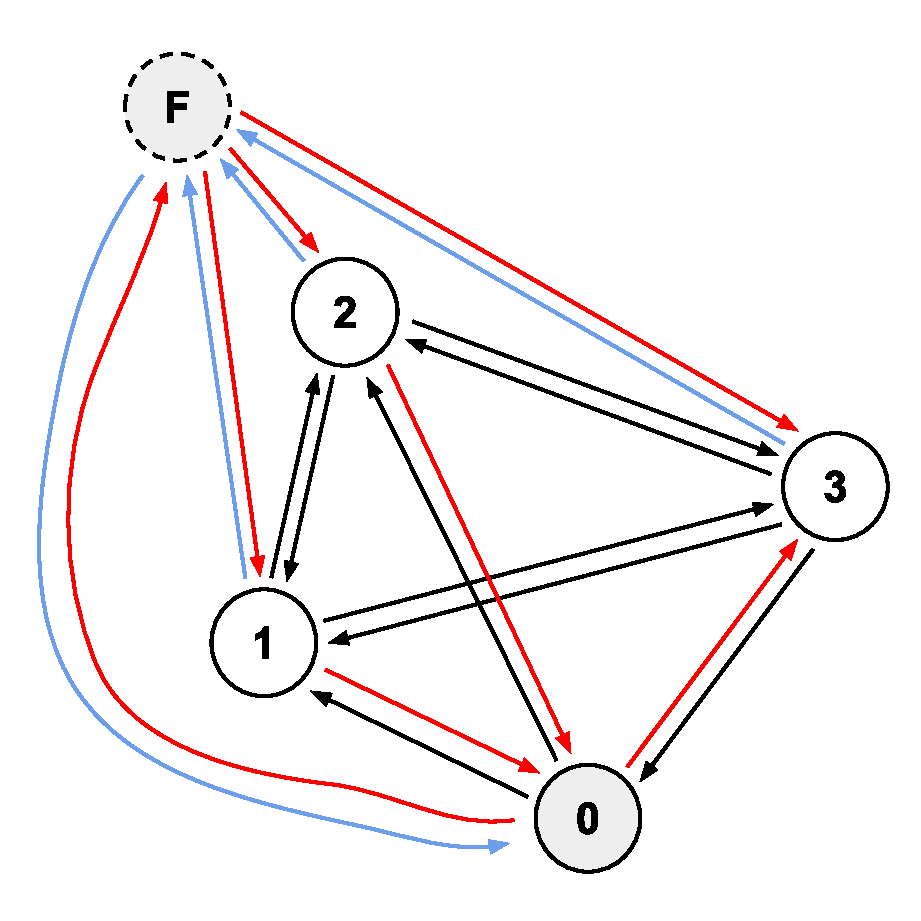
\includegraphics[width=0.4\textwidth]{./fig/photos/TSP.eps}
    \caption{An illustration of the modified distance matrix $\mathbf{D}_{mod}$ for the \ac{TSP} solver, that finds the optimal sequence of waypoints for each \ac{UAV}. 
    The vertex $v_{0}$ is the starting point of the sequence, vertices $\{v_{1}, v_{2}, v_{3}\}$ represent the waypoints to be visited by the \ac{UAV}, $v_{F}$ is an additional dummy virtual vertex. 
    The black edges represent the euclidean distance between corresponding vertices, the value of red edges is set to positive constant $M$, the value of blue edges is set to $0$. }
    \label{fig:tsp}
\end{figure}
%The modified distance matrix $\mathbf{D}_{mod}$ is then passed to the numerical solver.%%}

%%%%%%%%%%%%%%%%%%%%%%%
%%%% PATH PLANNING %%%%
%%%%%%%%%%%%%%%%%%%%%%%
\section{Path planning}% %%{
Once the sequence of waypoints for each \ac{UAV} is determined, the last step is a path planning.
The paths should be collision-free, the minimal distance between each pair of \ac{UAV}s should be at least $\SI{4}\meter$).
The planning method is based on astar planner implemented in the mrs uav system \cite{mrs_system}.
Each \ac{UAV} is assigned a certain priority.
The planning method is described in algorithm \autoref{alg:planning}.
The paths are planned sequentially for each drone based on its priority.
Once a path for a drone is generated, the inflated (by the safety distance radius $r = \SI{4}\meter$) points of the path are considered as obstacles for all drones with the lower priority.
If any of the waypoints is not reachable (for example some drone with higher priority planned path in close distance to it), the waypoint is skipped.
The path is then smoothed by the mrs uav system \cite{mrs_system} onboard the drone and executed by the drone's controller.






  \begin{algorithm}[!h]
  \caption{Multi-path planning}\label{alg:cap}
  \begin{algorithmic}

  \Function {plan\_paths}{$drones\_waypoints, drones\_poses$}
    \State $planned\_paths \gets \{\}$
    \For {$drone \in drones$} \Comment{iterate over drones based on priority}
      \State $obstacles \gets \{\}$
      \For {$path \in planned\_paths$}
        \State $obstacles \gets obstacles \cup \Call{inflate\_points}{path}$ %\Comment{mark positions around already planned paths as obstacles}
      \EndFor
      \State $path \gets \{\}$
      \State $segment\_start \gets drone\_pose$
      \For {$waypoint \in drone\_waypoints$}

        \If{ $waypoint \in obstacles$}
          \State \textbf{continue}
        \EndIf
        \State $path\_segment \gets \Call{astar\_planner}{start, waypoint, obstacles}$
        \State $segment\_start \gets waypoint$
        \State $path \gets path \cup path\_segment$
      \EndFor
      \State $planned\_paths \gets planned\_paths \cup path$
    \EndFor
    \State \Return $planned\_paths$
  \EndFunction


  \end{algorithmic}
    \label{alg:planning}
  \end{algorithm}% %%}


\subsection{Custom data message}
A custom \ac{ROS} message was developed to transfer necessary data from \ac{UAV} to the ground station.
The message consists of the \ac{ROS} header containing the coordinate frame (all drones share the same coordinate system given their gps origin),
timestamp specifying the time when it was created,
pose of the drone and its Compton camera 
and predicted point representing the future position of the \ac{UAV} in time horizon of $2$ seconds (which is generated by the \verb|mpc tracker| that is part of the mrs uav system \cite{mrs_system}).
The structure of the message is shown here:

\begin{lstlisting}[caption={DroneDataMsg.msg (caption)}, title={Custom message for data sharing between \ac{UAV} and central unit.}, label={code1}]
Header header
geometry_msgs/Pose pose
geometry_msgs/Pose sensor_pose
geometry_msgs/PointStamped predicted_point
std_msgs/String status
\end{lstlisting}


\mycomment{% %%{
  \subsection{Waypoint generation}
  s a first step, the $\lambda$ matrix (containing the current estimate of sources position) is processed by a local maximum filter. 
  The maximum filter works by sliding a window of a specified size over the $\lambda$.
  The central position of the sliding window is highlighted as local maxima if it is greater than all other values in the sliding window.

  Each waypoint (local maxima) is assigned with a weight $w$.
  The weight is defined as follows:
  \begin{equation}
    w_{j} = \frac{\lambda_{j}}{s_{j_{normalised}}}
  \end{equation},
  where $s_{j_{normalised}} = \frac{s_{j}}{\max_{J}( s_{j})}$ is a sensitivity value for given position $s_{j}$ divided by.
  Such formulation of $w_{j}$ prioritise the points with the highest current estimate of ionizing radiation, that are less explored (have lower sensitivity).

  \begin{algorithm}
  \caption{Planning pipeline}\label{alg:cap}
  \begin{algorithmic}
    \State $POI \gets \Call{get\_points\_of\_interest}$
    \State $POI_{sorted} \gets \Call{filter\_points}{POI}$
    \State $POI_{exploration} \gets \Call{get\_unexplored\_area\_points}$
    
    \State $future\_poses \gets \Call{get\_future\_drone\_poses}$

    \State $W_{exploitation} \gets \Call{clustering}{future\_poses}$
    \State $W_{exploration} \gets \Call{clustering}{future\_poses}$
    
    \State
  \end{algorithmic}
  \end{algorithm}



}% %%}


